\section{Spulen in der Praxis - Transformator}
\subsection{Aufbau eines Transformators}
\begin{frame}
    \makeframetitle
    \begin{columns}
        \column{0.5\textwidth}
        \begin{itemize}
            \item Zwei oder mehr Spulen mit $N$ Windungen
            \item Befinden sich auf einen \textit{gemeinsamen Ferrit-/Eisenkern}
            \item Aufteilung in \textbf{Primär}- und \textbf{Sekundärspule(n)}
        \end{itemize}

        \column{0.5\textwidth}
        \begin{figure}
            \begin{center}
                \includegraphics[height=0.7\textwidth]{transformer.jpg}
            \end{center}
            \caption{Bild eines Transformators mit Eisenkern\cite{wiki_transformer}}
        \end{figure}

    \end{columns}
\end{frame}

\subsection{Eigenschaften und Funktionsweise eines Transformators}
\begin{frame}
    \makeframetitle
    \begin{itemize}
        \item Wird nahezu überall verwendet
        \item Erlaubt die \textit{Umwandlung von Spannungen}
        \item Funktioniert \alert{ausschließlich} mit Wechselspannung
    \end{itemize}

    \begin{figure}
        \begin{center}
            \begin{circuitikz}
                \draw
                (0, 0) node[transformer core](T){};
            \end{circuitikz}
        \end{center}
        \caption{Schaltkreiszeichen eines Transformators mit Eisenkern}
    \end{figure}
\end{frame}

\begin{frame}
    \makeframetitle
    \begin{itemize}
        \item An der Primärspule liegt eine \textit{Wechsel}spannung $U_P$ an
        \item Die Primärspule \textit{induziert} eine Wechselspannung $U_S$ an
            der Sekundärspule
        \item Für einen \textit{idealen} und \textit{unbelasteten}
            Transformator gilt: \\
            $\frac{U_S}{U_P} = \frac{N_S}{N_P}$
    \end{itemize}
    \pause
    \begin{exampleblock}{Beispiel}
        geg.: $N_P = 5; N_S=10; U_P = 10V$
        \pause
        \begin{align}
            \frac{U_S}{U_P} &= \frac{N_S}{N_P} | \cdot U_P \\
            U_S &= \frac{N_S}{N_P} \cdot U_P \\ 
            \Rightarrow U_S &= \frac{10}{5} \cdot 10\unit\volt =
            \underline{20\unit\volt}
        \end{align}
    \end{exampleblock}
\end{frame}

\begin{frame}
\makeframetitle
\begin{figure}
    \begin{columns}
        \column{0.5\textwidth}
        \begin{center}
            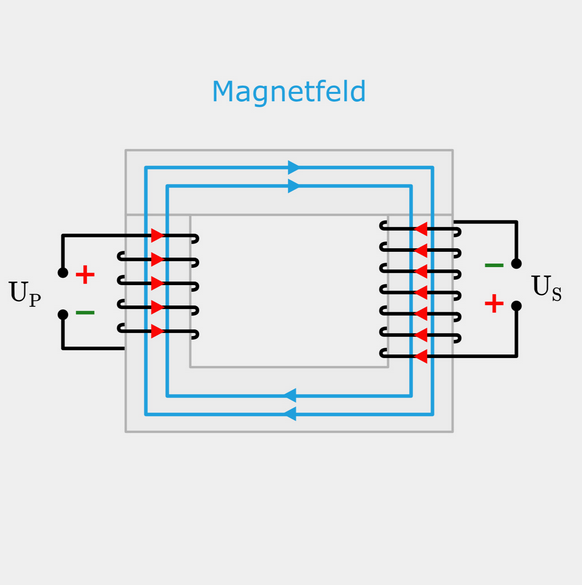
\includegraphics[height=0.80\textheight]{trans_ani1.jpg}
        \end{center}
        \column{0.5\textwidth}
        \caption{LEIFIphysik Animation\cite{leifi_trans_ani1}}
    \end{columns}
\end{figure}
\end{frame}

\subsection{Weitere Verwendungen von Spulen}
\begin{frame}
    \makeframetitle
    \begin{columns}
        \column{0.6\textwidth}
        \begin{itemize}
            \item Elektromotoren
            \item Relais
            \item Lautsprecher
            \item Elektromagneten
            \item Stromflussglättung
            \item usw...
        \end{itemize}
        \column{0.4\textwidth}
        \begin{figure}
            \begin{center}
                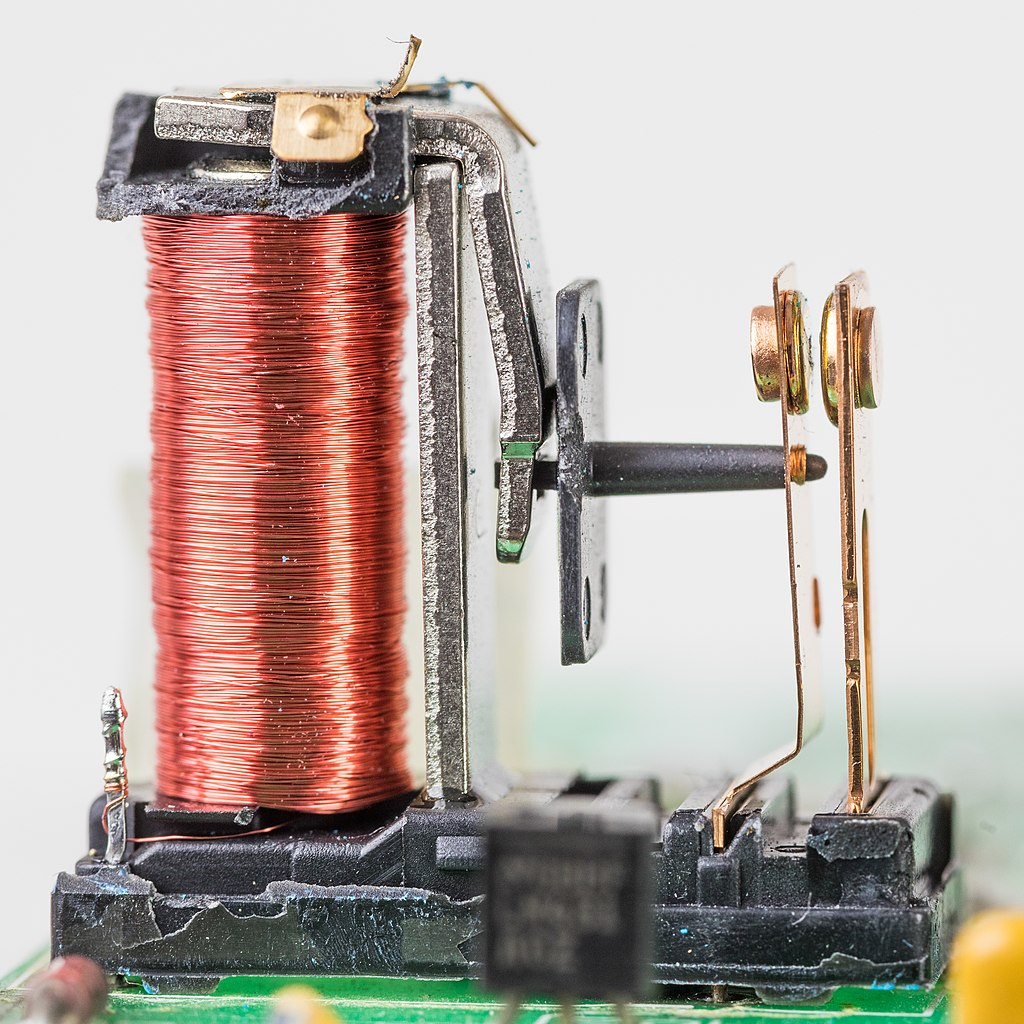
\includegraphics[width=0.9\textwidth]{relais.jpg}
            \end{center}
            \caption{Bild eines Relais\cite{wiki_relais}}
        \end{figure}
        
    \end{columns}
\end{frame}
